\documentclass[journal, a4paper]{IEEEtran}

% some very useful LaTeX packages include:

%\usepackage{cite}      % Written by Donald Arseneau
                        % V1.6 and later of IEEEtran pre-defines the format
                        % of the cite.sty package \cite{} output to follow
                        % that of IEEE. Loading the cite package will
                        % result in citation numbers being automatically
                        % sorted and properly "ranged". i.e.,
                        % [1], [9], [2], [7], [5], [6]
                        % (without using cite.sty)
                        % will become:
                        % [1], [2], [5]--[7], [9] (using cite.sty)
                        % cite.sty's \cite will automatically add leading
                        % space, if needed. Use cite.sty's noadjust option
                        % (cite.sty V3.8 and later) if you want to turn this
                        % off. cite.sty is already installed on most LaTeX
                        % systems. The latest version can be obtained at:
                        % http://www.ctan.org/tex-archive/macros/latex/contrib/supported/cite/

\usepackage{graphicx}   % Written by David Carlisle and Sebastian Rahtz
                        % Required if you want graphics, photos, etc.
                        % graphicx.sty is already installed on most LaTeX
                        % systems. The latest version and documentation can
                        % be obtained at:
                        % http://www.ctan.org/tex-archive/macros/latex/required/graphics/
                        % Another good source of documentation is "Using
                        % Imported Graphics in LaTeX2e" by Keith Reckdahl
                        % which can be found as esplatex.ps and epslatex.pdf
                        % at: http://www.ctan.org/tex-archive/info/

%\usepackage{psfrag}    % Written by Craig Barratt, Michael C. Grant,
                        % and David Carlisle
                        % This package allows you to substitute LaTeX
                        % commands for text in imported EPS graphic files.
                        % In this way, LaTeX symbols can be placed into
                        % graphics that have been generated by other
                        % applications. You must use latex->dvips->ps2pdf
                        % workflow (not direct pdf output from pdflatex) if
                        % you wish to use this capability because it works
                        % via some PostScript tricks. Alternatively, the
                        % graphics could be processed as separate files via
                        % psfrag and dvips, then converted to PDF for
                        % inclusion in the main file which uses pdflatex.
                        % Docs are in "The PSfrag System" by Michael C. Grant
                        % and David Carlisle. There is also some information
                        % about using psfrag in "Using Imported Graphics in
                        % LaTeX2e" by Keith Reckdahl which documents the
                        % graphicx package (see above). The psfrag package
                        % and documentation can be obtained at:
                        % http://www.ctan.org/tex-archive/macros/latex/contrib/supported/psfrag/

%\usepackage{subfigure} % Written by Steven Douglas Cochran
                        % This package makes it easy to put subfigures
                        % in your figures. i.e., "figure 1a and 1b"
                        % Docs are in "Using Imported Graphics in LaTeX2e"
                        % by Keith Reckdahl which also documents the graphicx
                        % package (see above). subfigure.sty is already
                        % installed on most LaTeX systems. The latest version
                        % and documentation can be obtained at:
                        % http://www.ctan.org/tex-archive/macros/latex/contrib/supported/subfigure/

\usepackage{url}        % Written by Donald Arseneau
                        % Provides better support for handling and breaking
                        % URLs. url.sty is already installed on most LaTeX
                        % systems. The latest version can be obtained at:
                        % http://www.ctan.org/tex-archive/macros/latex/contrib/other/misc/
                        % Read the url.sty source comments for usage information.

%\usepackage{stfloats}  % Written by Sigitas Tolusis
                        % Gives LaTeX2e the ability to do double column
                        % floats at the bottom of the page as well as the top.
                        % (e.g., "\begin{figure*}[!b]" is not normally
                        % possible in LaTeX2e). This is an invasive package
                        % which rewrites many portions of the LaTeX2e output
                        % routines. It may not work with other packages that
                        % modify the LaTeX2e output routine and/or with other
                        % versions of LaTeX. The latest version and
                        % documentation can be obtained at:
                        % http://www.ctan.org/tex-archive/macros/latex/contrib/supported/sttools/
                        % Documentation is contained in the stfloats.sty
                        % comments as well as in the presfull.pdf file.
                        % Do not use the stfloats baselinefloat ability as
                        % IEEE does not allow \baselineskip to stretch.
                        % Authors submitting work to the IEEE should note
                        % that IEEE rarely uses double column equations and
                        % that authors should try to avoid such use.
                        % Do not be tempted to use the cuted.sty or
                        % midfloat.sty package (by the same author) as IEEE
                        % does not format its papers in such ways.

\usepackage{amsmath}    % From the American Mathematical Society
                        % A popular package that provides many helpful commands
                        % for dealing with mathematics. Note that the AMSmath
                        % package sets \interdisplaylinepenalty to 10000 thus
                        % preventing page breaks from occurring within multiline
                        % equations. Use:
%\interdisplaylinepenalty=2500
                        % after loading amsmath to restore such page breaks
                        % as IEEEtran.cls normally does. amsmath.sty is already
                        % installed on most LaTeX systems. The latest version
                        % and documentation can be obtained at:
                        % http://www.ctan.org/tex-archive/macros/latex/required/amslatex/math/
\usepackage{listings}

\usepackage{xcolor}


% Other popular packages for formatting tables and equations include:

%\usepackage{array}
% Frank Mittelbach's and David Carlisle's array.sty which improves the
% LaTeX2e array and tabular environments to provide better appearances and
% additional user controls. array.sty is already installed on most systems.
% The latest version and documentation can be obtained at:
% http://www.ctan.org/tex-archive/macros/latex/required/tools/

% V1.6 of IEEEtran contains the IEEEeqnarray family of commands that can
% be used to generate multiline equations as well as matrices, tables, etc.

% Also of notable interest:
% Scott Pakin's eqparbox package for creating (automatically sized) equal
% width boxes. Available:
% http://www.ctan.org/tex-archive/macros/latex/contrib/supported/eqparbox/

% *** Do not adjust lengths that control margins, column widths, etc. ***
% *** Do not use packages that alter fonts (such as pslatex).         ***
% There should be no need to do such things with IEEEtran.cls V1.6 and later.


% Your document starts here!
\begin{document}
\begin{titlepage}

\newcommand{\HRule}{\rule{\linewidth}{0.5mm}} % Defines a new command for the horizontal lines, change thickness here

\center % Center everything on the page
 %----------------------------------------------------------------------------------------
%	LOGO SECTION
%----------------------------------------------------------------------------------------

~\\[1cm]

\includegraphics{SCUT.png}\\[2cm] % Include a department/university logo - this will require the graphicx package

%----------------------------------------------------------------------------------------
%	TITLE SECTION
%----------------------------------------------------------------------------------------

\HRule \\[1cm]
{ \huge \bfseries The Experiment Report of \textit{Machine Learning} }\\[0.6cm] % Title of your document
\HRule \\[2cm]
%----------------------------------------------------------------------------------------
%	HEADING SECTIONS
%----------------------------------------------------------------------------------------


\textsc{\LARGE \textbf{School:} School of Software Engineering}\\[1cm]
\textsc{\LARGE \textbf{Subject:} Software Engineering}\\[2cm] 

 
%----------------------------------------------------------------------------------------
%	AUTHOR SECTION
%----------------------------------------------------------------------------------------

\begin{minipage}{0.4\textwidth}
\begin{flushleft} \large
\emph{Author:}\\
 Chen Han % Your name
\end{flushleft}
\end{minipage}
~
\begin{minipage}{0.4\textwidth}
\begin{flushright} \large
\emph{Supervisor:} \\
Mingkui Tan% Supervisor's Name
\end{flushright}
\end{minipage}\\[2cm]
~
\begin{minipage}{0.4\textwidth}
\begin{flushleft} \large
\emph{Student ID:}\\
201936380086
\end{flushleft}
\end{minipage}
~
\begin{minipage}{0.4\textwidth}
\begin{flushright} \large
\emph{Grade:} \\
Class 1, Grade 2019
\end{flushright}
\end{minipage}\\[2cm]

% If you don't want a supervisor, uncomment the two lines below and remove the section above
%\Large \emph{Author:}\\
%John \textsc{Smith}\\[3cm] % Your name

%----------------------------------------------------------------------------------------
%	DATE SECTION
%----------------------------------------------------------------------------------------

{\large \today}\\[2cm] % Date, change the \today to a set date if you want to be precise

 
%----------------------------------------------------------------------------------------

\vfill % Fill the rest of the page with whitespace

\end{titlepage}

% Define document title and author
	\title{Linear Regression and Stochastic Gradient Descent}
	\maketitle

% Write abstract here
\begin{abstract}
Further understand of linear regression ,closed-form solution and Stochastic gradient descent with experiments.
\end{abstract}

% Each section begins with a \section{title} command
\section{Introduction}
	% \PARstart{}{} creates a tall first letter for this first paragraph
\PARstart{I}{n} order to further understand the conception of linear regression and stochastic gradient descent, we calculate the closed-form solution of linear regression and act stochastic gradient descent on a small dataset, conducted optimized parameter and observed the experimental effect.

% Main Part
\section{Methods and Theory}
We use linear regression and stochastic gradient descent. 

 Linear regression tries to learn a linear model to predict the output as best as possible.  More generally, we try to learn a model like : 
 $$ f(\boldsymbol{x}_i) = \boldsymbol{w}^T\boldsymbol{x}_i +b $$
 which is called multiple linear model.\par
 \subsection{first part}
 The first part of this experiment is to obtain the closed-form solution of linear regression. There are the steps:
\\1. Determine the loss function of this linear regression:\\

\begin{equation}
	\begin{aligned}
Loss(\boldsymbol{w})&=\frac{1}{2}\sum_{i=1}^{n}{(y_i-\boldsymbol{x}_i\boldsymbol{w})^2}\\
&=\frac{1}{2}\begin{bmatrix}y_1-\boldsymbol{x}_1\boldsymbol{w} \\ \vdots \\  y_n-\boldsymbol{x}_n\boldsymbol{w}\end{bmatrix}^T\begin{bmatrix}y_1-\boldsymbol{x}_1\boldsymbol{w} \\ \vdots \\  y_n-\boldsymbol{x}_n\boldsymbol{w} \\ 
    \end{bmatrix}\\ \nonumber
&=\frac{1}{2}(\boldsymbol{y-Xw})^T(\boldsymbol{y-Xw})
	\end{aligned}
\end{equation}
\\
where 
\begin{equation}
	\begin{aligned}
\boldsymbol{x}_i &=(x_{11},x_{12},\cdots,x_{1m},1)\boldsymbol{w}\\
&                 =(w_1,w_2,\cdots,w_m,b)^T \boldsymbol{X}\\ \nonumber
&                 =(\boldsymbol{x_1},\cdots,\boldsymbol{x_n})^T\\
	\end{aligned}
\end{equation}	

2. Take the derivative of the loss function:\\
 $$\boldsymbol{ a= y-Xw}$$

\begin{eqnarray}
\nonumber
    \frac{\partial{Loss(\boldsymbol{w})}}{\partial{\boldsymbol{w}}}&=&\frac{\partial \boldsymbol{a}}{\partial\boldsymbol{w}}\frac{\partial{(\frac{1}{2}\boldsymbol{a}^T\boldsymbol{a})}}{{\partial \boldsymbol{a}}}\\ \nonumber
    &=&\frac{1}{2}\frac{\partial{\boldsymbol{a}}}{\partial{\boldsymbol{w}}}(2\boldsymbol{a})\\ \nonumber
    &=&\frac{\partial {(\boldsymbol{y-Xw})}}{\partial\boldsymbol{w}}(\boldsymbol{y-Xw})\\ \nonumber
    &=&\boldsymbol{-X^T(y-Xw)}
\end{eqnarray}

3. Since Loss($\boldsymbol{w}$) is a convex function, we can get $\boldsymbol {w^*}$ from $\frac{\partial{Loss(\boldsymbol{w})}}{\partial{\boldsymbol{w}}}=0 $

$$\boldsymbol{w^*=(X^TX)^{-1}X^TY}$$

\subsection{second part}
\par The second part of this experiment is to obtain the linear regression model through the method of stochastic gradient descent. \par In machine learning algorithms, it is sometimes necessary to build a loss function for the original model, and then optimize the loss functionthrough the optimization algorithm, so as to find the optimal parameters and minimize the value of the loss function. In the optimization algorithm of machine learning parameters, the algorithm based on gradient descent(GD)is often used.
\par Stochastic gradient descent (SGD) is a simple but very effective method, which is widely used for linear classifier learning under convex loss functions such as SVMs and logistic regression.
\par There are the steps:
\\1. Find the best direct D. We can use $\boldsymbol{D}=-\frac{\partial{Loss(\boldsymbol{w})}}{\partial\boldsymbol{w}} $ as the direction optimization.
    $$\boldsymbol{D_{t}=-x_i^T(y-x_tw_t)}$$
    where $\boldsymbol{x_t}$ is a random sample in train set.
\\2. Find a good step size $\eta$ which is called it learning rate.
\\3. Set $\boldsymbol{w_{t+1}=w_t}+\eta\boldsymbol{D_t}$
\\4. Repeat step 1,2,3 for 5 to 8 rounds.

\section{Experiments}
\subsection{Dataset}
Linear Regression uses Housing in LIBSVM Data, including 506 samples and each sample has 13 features. We split the dataset by 75\% for training and 25\% for validation.

\subsection{Implementation}

	% You can reference tables and figure by using the \ref{label} command. Each table and figure needs to have a UNIQUE label.
	

	% This is how you define a table: the [!hbt] means that LaTeX is forced (by the !) to place the table exactly here (by h), or if that doesnt work because of a pagebreak or so, it tries to place the table to the bottom of the page (by b) or the top (by t).

1. Load the experiment data. You can use load\_svmlight\_file function in sklearn library.\par
2. Devide dataset by 0.25.\par
3. write Loss-calculating function.\par

\lstset{language=python}
\lstset{
	breaklines,
    numbers=left, 
    numberstyle= \tiny, 
    keywordstyle= \color{ blue!70},
    commentstyle= \color{red!50!green!50!blue!50}, 
    frame=shadowbox,
    rulesepcolor= \color{ red!20!green!20!blue!20} ,
    escapeinside=``, 
    xleftmargin=2em, aboveskip=1em,
    framexleftmargin=2em
}


\begin{lstlisting}
def calc_loss(X, y, W):
    loss = 0.5*(np.linalg.norm(y-X.dot(W))**2)
    return loss
\end{lstlisting}

4. Get the closed-form solution by formula:
$$W^* = (X^T X)^{-1} X^T Y$$\par
\begin{lstlisting}
def solve_W_closed_form(X, Y):
    Y = np.array(Y)
    W = np.linalg.inv(X.T.dot(X)).dot(X.T).dot(Y)
    return W
\end{lstlisting}

5. write stochastic gradient descent function.
\begin{lstlisting}
def solve_W_stochastic_gradient_descent(X, Y, learning_rate, epoch, batch, X_test, Y_test):
    train_loss = []
    test_loss = []
    Y = Y.reshape(Y.shape[0], 1)
    W = np.random.rand(X.shape[1], 1)
    for i in range(epoch):
        bat = np.random.choice(X.shape[0], batch)
        X_batch = X[bat]
        Y_batch = Y[bat]
        gradient = -X_batch.T.dot(Y_batch) + X_batch.T.dot(X_batch).dot(W)
        gradient = gradient * (1/batch)
        # normnazie
        W = W - learning_rate * gradient
        epoch_train_loss = calc_loss(X, Y, W)
        epoch_test_loss = calc_loss(X_test, Y_test, W)
        train_loss.append(epoch_train_loss)
        test_loss.append(epoch_test_loss)
    #print(loss)
    return W,train_loss, test_loss
\end{lstlisting}

\par
6. Get the solution.

	\begin{table}[!hbt]
		% Center the table
		\begin{center}
		% Title of the table
		\caption{value of $loss$ in linear regression}
		\label{tab:simParameters}
		% Table itself: here we have two columns which are centered and have lines to the left, right and in the middle: |c|c|
		\begin{tabular}{|c|c|}
			% To create a horizontal line, type \hline
			\hline
			% To end a column type &
			% For a linebreak type \\
			$Loss$ value& $5636.7082077152245$ \\
			\hline
			$Loss\_train$ value & $4233.440988955715$ \\
			\hline
			$Loss\_val$ value & $1403.2672187595103$\\
			\hline
		\end{tabular}
		\end{center}
	\end{table}

	% If you have questions about how to write mathematical formulas in LaTeX, please read a LaTeX book or the 'Not So Short Introduction to LaTeX': tobi.oetiker.ch/lshort/lshort.pdf
	\begin{table}[!hbt]
		% Center the table
		\begin{center}
		% Title of the table
		\caption{value of $loss$ in stochastic gradient descent}
		\label{tab:simParameters}
		% Table itself: here we have two columns which are centered and have lines to the left, right and in the middle: |c|c|
		\begin{tabular}{|c|c|}
			% To create a horizontal line, type \hline
			% To end a column type &
			% For a linebreak type \\
			\hline
			$Loss\_train$ value & $5049.16020020202$ \\
			\hline
			$Loss\_val$ value & $1780.4511281009281$\\
			\hline
		\end{tabular}
		\end{center}
	\end{table}


	% This is how you include a eps figure in your document. LaTeX only accepts EPS or TIFF files.
	\begin{figure}[!hbt]
		% Center the figure.
		\begin{center}
		% Include the eps file, scale it such that it's width equals the column width. You can also put width=8cm for example...
		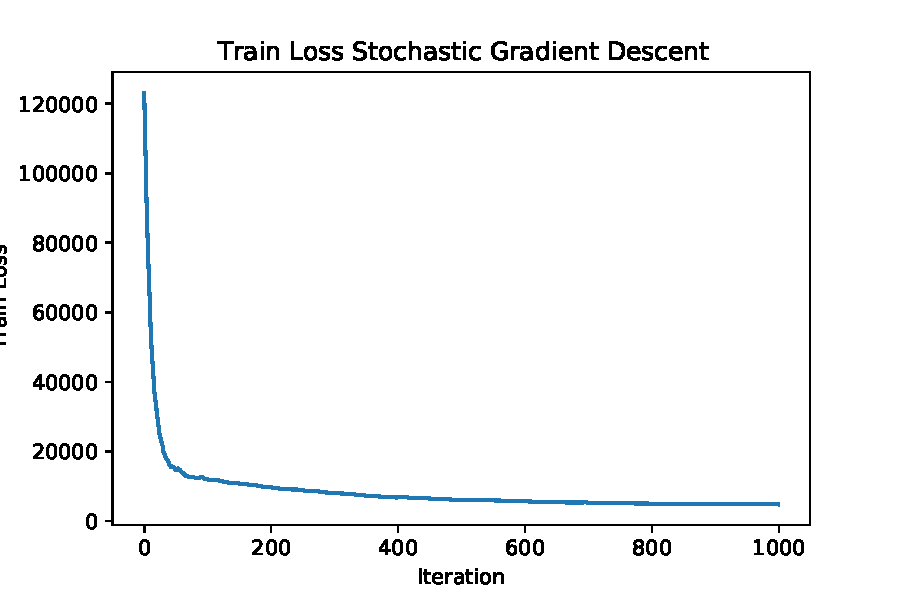
\includegraphics[width=\columnwidth]{lab1_sto_sam_train}
		% Create a subtitle for the figure.
		\caption{Train Loss Stochastic Gradient Descent.}
		% Define the label of the figure. It's good to use 'fig:title', so you know that the label belongs to a figure.
		\end{center}
	\end{figure}
		% This is how you include a eps figure in your document. LaTeX only accepts EPS or TIFF files.
	\begin{figure}[!hbt]
		% Center the figure.
		\begin{center}
		% Include the eps file, scale it such that it's width equals the column width. You can also put width=8cm for example...
		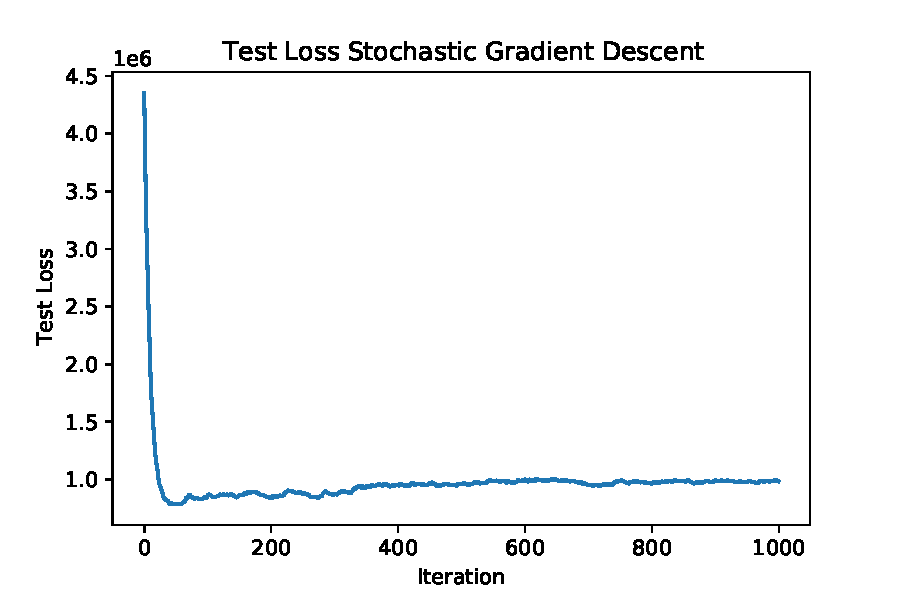
\includegraphics[width=\columnwidth]{lab1_sto_sam_test}
		% Create a subtitle for the figure.
		\caption{validation Loss Stochastic Gradient Descent.}
		% Define the label of the figure. It's good to use 'fig:title', so you know that the label belongs to a figure.
		\end{center}
	\end{figure}


\section{Conclusion}
	In this experiment, I learnt to use linear regression and stochastic gradient descent. Also, I review coding with python and realize the advantage of LaTeX.



% Your document ends here!
\end{document}